% \documentclass[handout]{beamer}
\documentclass[hyperref={pdftex,unicode}]{beamer}
\usepackage{pgfpages}
% \pgfpagesuselayout{4 on 1}[a4paper,border shrink=10mm,landscape]



\usepackage[T2A]{fontenc}
\usepackage[utf8]{inputenc}
\usepackage[russian]{babel}
\usepackage{amsmath}
\usepackage{amsfonts}
\usepackage[warn]{mathtext}
\usepackage{graphicx}
\newcommand*{\hm}[1]{#1\nobreak\discretionary{}%
 {\hbox{$\mathsurround=0pt #1$}}{}}

\graphicspath{{./pictures/}}
\usepackage{type1cm}
\usepackage{type1ec}
\usepackage{tabularx}
\usepackage{caption}
% \usepackage{textgreek}
\usepackage{xcolor}

\usetheme{Madrid}
\usecolortheme{spruce}
% \usecolortheme{dolphin}
\useinnertheme{rectangles}
%\usecolortheme{whale}
\graphicspath{{./pictures/}}
\setbeamercolor{alerted text}{fg=red} 
\setbeamerfont{alerted text}{series=\bfseries}
\usepackage{tikz}
\newcommand*\circled[1]{\tikz[baseline=(char.base)]{
            \node[shape=circle,draw,inner sep=2pt] (char) {#1};}}
\setbeamertemplate{navigation symbols}{}
% Листинги
\usepackage{listings}
\lstdefinestyle{verilog}{
  extendedchars={true},
  inputencoding={utf8},
  language={Verilog},
  basicstyle={\ttfamily \tiny},
  keywordstyle={\rmfamily \bfseries},
  commentstyle={\rmfamily \itshape},
  tabsize={2},
  frame={single},
  showstringspaces={false},
  breaklines={true},
}
\lstdefinestyle{xml}{
  extendedchars={true},
  inputencoding={utf8},
  language={XML},
  basicstyle={\ttfamily \tiny},
  keywordstyle={\rmfamily \bfseries},
  commentstyle={\rmfamily \itshape},
  tabsize={2},
  frame={single},
  showstringspaces={false},
  breaklines={true},
}
\lstdefinestyle{cpp}{
  extendedchars={true},
  inputencoding={utf8},
  language={C++},
  basicstyle={\ttfamily \scriptsize},
  keywordstyle={\rmfamily \bfseries},
  commentstyle={\rmfamily \itshape},
  tabsize={2},
  numbers={none},
  frame={single},
  showstringspaces={false},
  breaklines={true},
}

\lstdefinestyle{base}{
  language=Java,
  emptylines=1,
  breaklines=true,
  basicstyle=\ttfamily\color{black},
  moredelim=**[is][\color{red}]{@}{@},
  showstringspaces=false,
}

\begin{document}
	
% \setbeamertemplate{navigation symbols}{}
% \setbeamertemplate{footline}{%
% 	\hspace{0.94\paperwidth}%
% 	\usebeamerfont{title in head/foot}%
% 	\insertframenumber\,/\,\inserttotalframenumber%
% }
% \title{Разработка аспектно-ориентированного расширения для языка Kotlin}
	
% \author{
% 	Скрипаль Б.А.\\
% 	Ицыксон В.М.\\
% }
% \institute[СПбПУ]{Санкт-Петербургский политехнический университет Петра Великого}
% \date[21.04.2017]{21 апреля 2017}  
% % Создание заглавной страницы
% \frame{\titlepage} 
\title[АОП-расширение для Kotlin]
{Разработка аспектно-ориентированного расширения для языка Kotlin}
\author[Скрипаль Б.]{{\bf Скрипаль~Б.А.} \and Ицыксон~В.М.}
\date[21.04.2017]{21 апреля 2017 г.}

\institute[СПбПУ]{Санкт-Петербургский политехнический университет Петра Великого }	
\maketitle
\begin{frame}[fragile=singleslide]
	\frametitle{Введение}
	\begin{itemize}
		\item Аспектно-ориентированный подход позволяет описывать и
		      внедрять сквозную функциональность
		\item Представлен в 1997 году Грегором Кичалесом
		\item Используется совместно с объектно-ориентированным подходом
	\end{itemize}
\end{frame}

\begin{frame}[fragile=singleslide]
	\frametitle{Задачи, решаемые АОП}
	\begin{itemize}
		\item Протоколирование
		\item Обработка ошибок
		\item Проверка прав доступа
		\item Проверка пост- и предусловий
		\item Трассировка
		\item ...
	\end{itemize}
\end{frame}

\begin{frame}[fragile=singleslide]
	\frametitle{Реализации АОП для языков программирования}
	\begin{columns}
		\begin{column}{0.5\textwidth}
			\begin{itemize}
				\item Java
				      \begin{itemize}
				      	\item Spring AOP
				      	\item Aspect
				      	\item JAML
				      	\item CaesarJ
				      	\item ...
				      \end{itemize}
				\item C\#
				      \begin{itemize}
				      	\item PostSharp
				      	\item Aspect.NET
				      	\item AspectC\#
				      	\item ...
				      \end{itemize}
			\end{itemize}
		\end{column}
		\begin{column}{0.5\textwidth}  %%<--- here
			\begin{itemize}
				\item Python
				      \begin{itemize}
				      	\item Aspyct
				      	\item PyPy
				      	\item PEAK
				      	\item Lightweight Python AOP
				      	\item ...
				      \end{itemize}
				      
				\item C/C++
				      \begin{itemize}
				      	\item AspectC
				      	\item AspectC++
				      	\item FeatureC++
				      	\item ...
				      \end{itemize}
				      
			\end{itemize}
		\end{column}
	\end{columns}

	\begin{center}
	\Huge Kotlin?
	\end{center}
				
\end{frame}


\begin{frame}[fragile=singleslide]
	\frametitle{Основные понятия}
	\begin{itemize}
		\item Аспект (aspect) --- сущность, инкапсулирующая в себе сквозную
		      функциональность
		\item Точка внедрения (join point) --- точка в программе, к которой
		      должна быть применена сквозная функциональность
		\item Срез (pointcut) --- множество всех точек внедрения, к которым
		      должна быть применена сквозная функциональность
		\item Совет (advice) --- сущность, содержащая функциональность,
		      которая должна быть применена к точке внедрения
		      
	\end{itemize}
\end{frame}	
	

\begin{frame}[fragile=singleslide]
	\frametitle{Способы описания аспектов}
	\begin{itemize}
		\item Аннотации
		\item Расширения целевого языка
		\item Аннотирующие комментарии
		\item Специальные классы
		\item XML
		\item ...
	\end{itemize}
\end{frame}


\begin{frame}[fragile=singleslide]
	\frametitle{Способы внедрения сквозной функциональности}
	\begin{itemize}
		\item Статический:
		      \begin{itemize}
		      	\item На уровне исходных кодов
		      	\item Во время компиляции
		      	\item Сразу после компиляции
		      \end{itemize}
		\item Динамический:
		      \begin{itemize}
		      	\item При помощи прокси-объектов
		      	\item Во время загрузки файлов в JVM
		      	\item ...
		      \end{itemize}
	\end{itemize}
\end{frame}
\begin{frame}[fragile=singleslide]
	\frametitle{Описание аспектов для Kotlin}
	

	
	\begin{itemize}
		\item База --- AspectJ
		\item Адаптация под особенности языка Kotlin
	\end{itemize}

	% \begin{itemize}
	% 	\item Популярность AspectJ
	% 	\item Удобство и наглядность
	% 	\item Грамматика синтаксиса AspectJ находится в открытом доступе
	% \end{itemize}
\end{frame}

\begin{frame}[fragile=singleslide]
	\frametitle{Адаптация синтаксиса AspectJ к языку Kotlin}
	\begin{itemize}
		\item Приведение описания функций к виду, используемому в Kotlin
		\item Изменение стандартных типов Java на типы Kotlin
		\item Изменение модификаторов полей и методов
		\item Добавление возможности задания атрибутов аргументов методов
		\item Добавление поддержки функций-расширений (extension
		      functions)
	\end{itemize}
\end{frame}

\begin{frame}[fragile=singleslide]
	\frametitle{Пример описания аспекта для языка Kotlin}
	\begin{lstlisting}[frame=single,style=base]
aspect A  {
    pointcut fooPC(): execution(fun Foo.*())
    pointcut printPC(): call(public !extension fun kotlin.io.pri*(Any?))

    before(): fooPC() && printPC() {
        println("Hello before!!")
    }

    after(): fooPC() && printPC() {
        println("Hello after!!")
    }
}
	\end{lstlisting}
\end{frame}

\begin{frame}[fragile=singleslide]
	\frametitle{Реализованные возможности}
			
	\begin{itemize}
		\item Вставка советов:
		      \begin{itemize}
		      	\item before
		      	\item after
		      	\item around
		      \end{itemize}
		\item Описание срезов:
		      \begin{itemize}
		      	\item call
		      	\item execution
		      \end{itemize}
		\item Поддержка extension функций
		\item Задание nullability модификаторов
	\end{itemize}
\end{frame}

\begin{frame}[fragile=singleslide]
	\frametitle{Внедрение аспектов}
	\framesubtitle{}
	Статический способ внедрения на уровне промежуточного представления
	
	\begin{enumerate}
		\item Построение PSI
		\item Построение модели аспектов
		\item Разметка элементов PSI тегами, соответствующим срезам
		\item Внедрение кода советов
		\item Компиляция PSI
	\end{enumerate}
\end{frame}

\begin{frame}[fragile=singleslide]
	\frametitle{Внедрение аспектов}
	\begin{figure}[h]
		\center{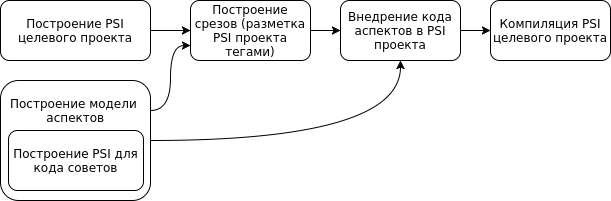
\includegraphics[width=1\linewidth]{../aspect_weaving.png}}
		\caption{Процесс внедрения аспектов}
		\label{ris:aspect_weaving}
	\end{figure}
\end{frame}


\begin{frame}[fragile=singleslide]
	\frametitle{Внедрение кода советов}
	При применении совета к вложенному вызову используем лямбда-wrapper <<run>>

	Выражение
	\begin{lstlisting}[frame=single,style=base]
val a = a.foo().bar()
	\end{lstlisting}
	преобразуется в:
	\begin{lstlisting}[frame=single,style=base]
val a = a.
	@run{@
		@val buf = @foo()
		@advice_code@
		@buf}@
	.bar()
	\end{lstlisting}
\end{frame}

\begin{frame}[fragile=singleslide]
	\frametitle{Пример аспекта}
	\begin{lstlisting}[frame=single,style=base]
aspect A  {
    pointcut fooPC(): execution(fun Foo.*())
    pointcut printPC(): call(public !extension fun kotlin.io.pri*(Any?))

    before(): fooPC() && printPC() {
        println("Hello before!!")
    }

    after(): fooPC() && printPC() {
        println("Hello after!!")
    }
}
	\end{lstlisting}
\end{frame}


\begin{frame}[fragile=singleslide]
	\frametitle{Пример применения аспектов}
	\begin{lstlisting}[frame=single,style=base]
class Foo {
  fun foo() {
@    run{@
@      val ____a = run{@
@        println("Hello before!!")@
        println("Hello foo!!")
@      }@
@      println("Hello after!!")@
@      ____a@
@    }@
  }

  fun bar() {
  	println("Hello bar!!")
  }
}
	\end{lstlisting}
\end{frame}

\begin{frame}[fragile=singleslide]
	\frametitle{Тестирование прототипа}
	\begin{itemize}
		\item Искусственные примеры
		\item Студенческие проекты (размер в несколько сотен строк)
	\end{itemize}
	
	Время применения советов к программе занимает до нескольких секунд
\end{frame}

\begin{frame}[fragile=singleslide]
	\frametitle{Дальнейшие исследования}
	\begin{itemize}
		\item Реализация возможностей, существующих в AspectJ
			\begin{itemize}
				\item Структуры описания срезов (args, cflow)
				\item Способы применения советов (afterthrowing, afterreturning)
				\item Описание функций и переменных внутри аспекта
				\item Обращение к аргументам функций
			\end{itemize}
		\item Учет возможностей Kotlin
			\begin{itemize}
				\item inline функции
				\item ...
			\end{itemize}
		\item Тестирование и отладка
			\begin{itemize}
				\item Улучшение тестов
				\item Увеличение размеров и сложности тестовых проектов
			\end{itemize}
	\end{itemize}
\end{frame}

\begin{frame}[fragile=singleslide]
	\frametitle{Контактные данные}
	\begin{center}
	{\Large Санкт-Петербургский политехнический университет Петра Великого, кафедра КСПТ}
	\newline
	\begin{itemize}
		\item Скрипаль Б.А. \textit{skripal@kspt.icc.spbstu.ru}
		\item Ицыксон В.М. \textit{vlad@icc.spbstu.ru}
	\end{itemize}
	\end{center}
\end{frame}
\end{document}